\section{Experiments of the paper}

% ============================================================
% SLIDE 19
% ============================================================
\begin{frame}[shrink=21]{Paper kiểm tra ba câu hỏi gì?}{Paper experiments \textperiodcentered\ Q1--Q3}
\begin{columns}[T,onlytextwidth]
\begin{column}{0.32\textwidth}
\begin{intuition}[Q1 \quad Accuracy]
  MAE và RMSE ở nhiều tầm dự báo; thấp hơn là tốt hơn.
\end{intuition}
\end{column}
\begin{column}{0.32\textwidth}
\begin{mathcard}[Q2 \quad Scalability]
  Wall-clock theo stream length và average computation time.
\end{mathcard}
\end{column}
\begin{column}{0.32\textwidth}
\begin{takeaway}[Q3 \quad Effectiveness]
  Latent dynamics, factors và diffusion có giúp diễn giải dữ liệu không?
\end{takeaway}
\end{column}
\end{columns}
\vspace{5mm}
\centering
{\small
\begin{tabular}{@{}llcc@{}}
  \toprule
  Loại dữ liệu & D-Tracker input window & Forecast horizons & Đơn vị\\
  \midrule
  GoogleTrends & $L_c=104$ & 13, 26, 39 & tuần\\
  Covid-19 & $L_c=56$ & 7, 14, 21 & ngày\\
  \bottomrule
\end{tabular}}
\vspace{4mm}
\begin{questioncard}
  \softlabel{BASELINES}\par
  DISMO \textperiodcentered\ FluxCube \textperiodcentered\ PatchTST \textperiodcentered\ Autoformer \textperiodcentered\ DeepAR \textperiodcentered\ LaST \textperiodcentered\ CoST\\[1mm]
  {\small Table 3 nhân mọi MAE/RMSE với $10^{-2}$; reproduction phải giữ đúng scale này.}
\end{questioncard}
\vspace{2mm}
\papersource{§5, Q1--Q3 và experimental protocol, p. 7.}
\end{frame}

% ============================================================
% SLIDE 20
% ============================================================
\begin{frame}[shrink=33]{Sáu thực nghiệm trên GoogleTrends và Covid-19}{Paper experiments \textperiodcentered\ data setup}
\centering
{\small
\begin{tabular}{@{}llp{7.0cm}l@{}}
  \toprule
  ID & Dataset & Keywords / signals & Shape $(t,k,l)$\\
  \midrule
  1 & Device & 8 thiết bị: Apple Watch, \ldots, iPhone & $(676,8,50)$\\
  2 & Pythonlib & 7 thư viện: matplotlib, \ldots, tensorflow & $(676,7,50)$\\
  3 & VoD & 7 dịch vụ: Apple TV, \ldots, youtube & $(676,7,50)$\\
  4 & Chatapp & 8 ứng dụng: facebook, \ldots, whatsapp & $(676,8,50)$\\
  5 & Language & 9 ngôn ngữ/công nghệ web & $(676,9,50)$\\
  6 & Covid-19 & new infected, new deceased & $(990,2,50)$\\
  \bottomrule
\end{tabular}}
\vspace{4mm}
\begin{columns}[T,onlytextwidth]
\begin{column}{0.48\textwidth}
\begin{intuition}[GoogleTrends]
  Search volume theo tuần, 2010--2022.
\end{intuition}
\end{column}
\begin{column}{0.48\textwidth}
\begin{mathcard}[Covid-19]
  Số ca theo ngày, Jan 2020--Sep 2022.
\end{mathcard}
\end{column}
\end{columns}
\vspace{3mm}
\begin{questioncard}
  Toàn bộ được normalize về min 0, max 1. Table 4 dùng shape \textbf{(time, keyword, location)}; equations dùng \textbf{(keyword, location, time)}.
\end{questioncard}
\vspace{2mm}
\begin{caution}[Chi tiết cần giữ khi reproduce]
  Prose ghi 48 countries còn Table 4 ghi dimension 50; slide không tự “sửa” mâu thuẫn này.
\end{caution}
\vspace{1mm}
\papersource{§5 Datasets, p. 7; Appendix B.1, Table 4, p. 11.}
\end{frame}

% ============================================================
% SLIDE 21
% ============================================================
\begin{frame}[shrink=30]{Q1 Accuracy --- D-Tracker dẫn đầu MAE trong thiết lập paper}{Paper experiments \textperiodcentered\ Table 3}
\centering
{\small
\begin{tabular}{@{}lccccc@{}}
  \toprule
  Dataset & $L_f$ & D-Tracker MAE & Best baseline & Baseline MAE & Giảm MAE\\
  \midrule
  Device & 26 & \textbf{0.90} & DISMO & 1.19 & 24.4\%\\
  Pythonlib & 26 & \textbf{0.32} & CoST & 0.45 & 28.9\%\\
  VoD & 26 & \textbf{0.59} & DISMO & 0.66 & 10.6\%\\
  Chatapp & 26 & \textbf{0.34} & DISMO & 0.48 & 29.2\%\\
  Language & 26 & \textbf{0.35} & Autoformer & 0.41 & 14.6\%\\
  Covid-19 & 14 & \textbf{0.70} & Autoformer & 1.18 & 40.7\%\\
  \bottomrule
\end{tabular}}
\vspace{3mm}
\begin{intuition}[Cách đọc bảng]
  Mọi MAE đều có scale \textbf{$\times10^{-2}$}. “Giảm MAE” được tính lại bằng $100(B-D)/B$ từ chính các giá trị Table 3; đây là phép tính trên số paper, không phải kết quả reproduce.
\end{intuition}
\vspace{3mm}
\begin{takeaway}[Kết quả đầy đủ paper báo cáo]
  D-Tracker có best MAE trên các datasets và horizons được đánh giá. Paper đồng thời nói RMSE nhạy với lỗi lớn; backup A4 giữ đủ 18 cặp MAE--RMSE của D-Tracker.
\end{takeaway}
\vspace{2mm}
\papersource{Table 3, p. 8; Q1 narrative, §5, p. 7.}
\end{frame}

% ============================================================
% SLIDE 22
% ============================================================
\begin{frame}[shrink=31]{Ablation --- mỗi thành phần giúp ở những dữ liệu khác nhau}{Paper experiments \textperiodcentered\ Figure 3}
\begin{columns}[c,onlytextwidth]
\begin{column}{0.59\textwidth}
  \centering
  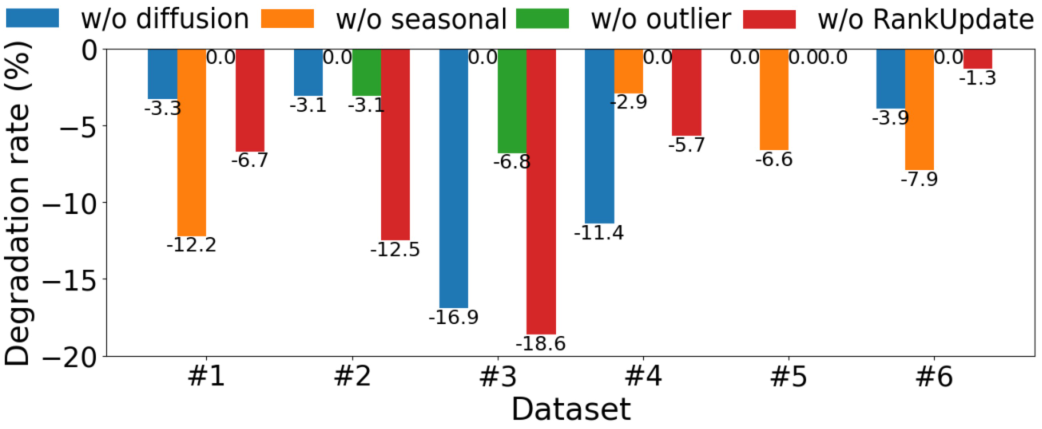
\includegraphics[width=\linewidth]{figures/drop_rate.png}\par
  {\scriptsize\color{DTMuted}Higashiguchi et al., KDD 2025, Figure 3 \textperiodcentered\ CC BY 4.0}
\end{column}
\begin{column}{0.38\textwidth}
  \begin{itemize}
    \item \textbf{Seasonal:} hữu ích ở Device, Language, Covid-19 --- các dữ liệu seasonality mạnh.
    \item \textbf{Diffusion:} cải thiện rõ ở VoD và Chatapp.
    \item \textbf{Outlier:} giúp một số dữ liệu bằng cách lọc abrupt changes.
    \item \textbf{RankUpdate:} thích nghi cấu trúc qua stream.
  \end{itemize}
  \vspace{2mm}
  \begin{caution}[Không phải lúc nào cũng giúp]
    Language không hưởng lợi từ diffusion. Seasonal/outlier cũng có thể không cải thiện khi những pattern này vắng mặt hoặc hiếm.
  \end{caution}
\end{column}
\end{columns}
\vspace{2mm}
{\small Ablation dùng horizon \textbf{26 tuần} hoặc \textbf{14 ngày}; so sánh full model với bỏ từng mechanism.}
\vspace{1mm}
\papersource{Figure 3 và discussion, §5 Q1, pp. 7--8.}
\end{frame}

% ============================================================
% SLIDE 23
% ============================================================
\begin{frame}[shrink=16]{Q2 Scalability --- tốc độ và RankUpdate spikes}{Paper experiments \textperiodcentered\ Figure 4}
\begin{columns}[T,onlytextwidth]
\begin{column}{0.37\textwidth}
\begin{takeaway}[Paper-reported speed-up]
  \centering
  {\fontsize{34}{38}\selectfont\bfseries\color{DTGold}up to 8.0$\times$\par}
  \vspace{2mm}
  {\large faster than competitors\par}
  \vspace{3mm}
  {\small Paper cũng báo cáo \textbf{fastest average time} trong Figure 4.}
\end{takeaway}
\end{column}
\begin{column}{0.60\textwidth}
\centering
\begin{tikzpicture}[x=.82cm,y=.60cm]
  \node[dtaccent,minimum width=4.5cm,minimum height=1.0cm,align=center] (window) at (2.5,2.0)
    {history dài dần\\nhưng window $L_c$ cố định};
  \node[dtbox,minimum width=3.5cm,minimum height=.95cm,align=center] (estimate) at (2.5,0)
    {ModelEstimation\\mỗi time step};
  \draw[dtarrow] (window)--(estimate);
  \node[dtgold,minimum width=4.2cm,minimum height=1.0cm,align=center] (rank) at (2.5,-2.0)
    {RankUpdate gọi lại nhiều lần\\$\Rightarrow$ runtime spikes};
  \draw[dtdash] (estimate)--(rank);
\end{tikzpicture}
\end{column}
\end{columns}
\vspace{3mm}
{\small Paper báo cáo fixed-window updates giúp processing time không tăng theo tổng stream length; không có nghĩa mọi phép toán là O(1).}
\vspace{2mm}

{\scriptsize\color{DTMuted}Nguồn: Figure 4/§5 Q2 p. 8 và speed-up claim §1 p. 3. Dense plots được thay bằng callout để dễ đọc khi chiếu.}
\end{frame}

% ============================================================
% SLIDE 24
% ============================================================
\begin{frame}[shrink=24]{Q3 Effectiveness --- đọc một diffusion pattern}{Paper experiments \textperiodcentered\ Figure 1(b), 2010--2011}
\begin{columns}[c,onlytextwidth]
\begin{column}{0.56\textwidth}
  \centering
  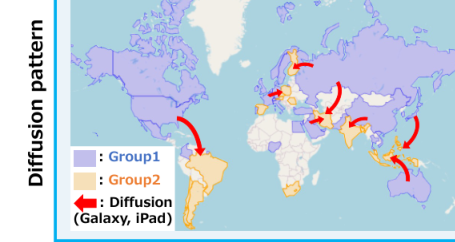
\includegraphics[width=\linewidth]{figures/Figure1b_diffusion_2010.png}\par
  {\scriptsize\color{DTMuted}Crop vùng diffusion 2010--2011 từ Figure 1(b), Higashiguchi et al., KDD 2025 \textperiodcentered\ CC BY 4.0}
\end{column}
\begin{column}{0.41\textwidth}
  \begin{itemize}
    \item $\mathcal W^{core}$: preview dùng 3 keyword groups × 2 location groups.
    \item $W^{key}$: Dynamics \#3 liên hệ Galaxy và iPad.
    \item $W^{loc}+\mathcal D$: paper diễn giải diffusion của Dynamics \#3 từ Group 1 sang Group 2 trong 2010--2011.
  \end{itemize}
\end{column}
\end{columns}
\vspace{3mm}
{\small \textbf{Cách đọc:} dynamics = chuyện gì diễn ra; factors = keyword/location liên hệ; reaction--diffusion = hướng liên hệ giữa nhóm.}
\vspace{2mm}
{\small\color{DTClaret}Structural interpretation trong model không phải causal experiment.}
\vspace{2mm}
\papersource{§1.1 và Figure 1(b), p. 2; effectiveness discussion, §5 Q3, p. 8.}
\end{frame}
